\todo[inline]{HTML Templates W3C Draft (18.März.2014) https://dvcs.w3.org/hg/webcomponents/raw-file/tip/spec/templates/index.html}
%http://www.w3.org/TR/html5/scripting-1.html#the-template-element

Um Web-Components besser verstehen zu können, wird in diesem Kapitel zu Beginn eine kurze Übersicht über die Geschichte von Web-Bibliotheken gezeigt.

\begin{description}
\item[2005] Veröffentlichung von Dojo Toolkit\footnote{Mehr Information zu Dojo Toolkit unter \href{http://dojotoolkit.org/}{http://dojotoolkit.org/}} mit der innovativen Idee von Widgets. Mit ein paar Zeilen Code konnten Entwickler komplexe Elemente, wie beispielsweise einen Graph oder eine Dialog-Box in ihrer Website hinzufügen.
\item[2006] jQuery\footnote{Mehr Information zu jQuery unter \href{http://jquery.com/}{http://jquery.com/}} stellt Entwicklern die Funktion zur Verfügung Plugins zu entwickeln, die später wiederverwendet werden können.
\item[2008] Veröffentlichung von jQuery UI\footnote{Mehr Information zu jQuery UI unter \href{http://jqueryui.com/}{http://jqueryui.com/}}, was vordefinierte Widgets und Effekte mit sich bringt.
\item[2009] Erstveröffentlichung von AngularJS\footnote{Mehr Information zu AngularJS unter \href{http://angularjs.org/}{http://angularjs.org/}}, ein Framework mit Direktiven.
\item[2011] Erstveröffentlichung von React\footnote{Mehr Information zu Facebook React unter \href{http://facebook.github.io/react/}{http://facebook.github.io/react/}}. Diese Bibliothek gibt den Entwicklern die Fähigkeit, das User Interface ihrer Website zu bauen, ohne dabei auf andere Frameworks, die auf der Seite benutzt werden, achten zu müssen
\item[2013] Veröffentlichung des Entwurfs von Web-Components, jedoch mit schlechter Browser Unterstützung
\end{description}

Mit der Veröffentlichung von Dojo Toolkit sagen Entwickler die Vorteile von wiederverwendbaren Modulen. Wenn man zurzeit Plugins auf einer Website erwähnt, denken die meisten Entwickler von jQuery Plugins, da sie beinahe überall Verwendung finden und ein großes Spektrum von Funktionen bieten. Mit den Veröffentlichungen von AngularJS und React wurde gezeigt, in welche Richtung sich Web-Anwendungen bewegen. Sie zeigen, dass es nicht nur um visuelle Elemente geht, sondern auch um Elemente, die eine komplexe Logik besitzen.




Ähnlich zu HTML5 ist Web-Components ein Sammelbegriff für mehrere Features:
\begin{description}
\item[Shadow DOM (ausführliche Erklärung siehe Kapitel \ref{sec:3_WC_Shadow_DOM} auf Seite \pageref{sec:3_WC_Shadow_DOM})] erlaubt es das DOM und CSS zu kapseln
\item[HTML Templates (ausführliche Erklärung siehe Kapitel \ref{sec:3_WC_Templates} auf Seite \pageref{sec:3_WC_Templates})] sind ein Weg, um den DOM zu klonen und somit den Klon wiederzuverwenden
\item[Custom Elements (ausführliche Erklärung siehe Kapitel \ref{sec:3_WC_Elements} auf Seite \pageref{sec:3_WC_Elements})] können einerseits neue Elemente definieren, oder bereits bestehende Elemente erweitern. Dies bedeutet, dass ein Entwickler beispielsweise den HTMl \lstinline|<input>|-Tag dahingehend erweitern kann, dass dieser nur das Format von Kreditkartennummern unterstützt. Ein Beispiel für die Definition eines neuen Elements wäre ein Element, dass sämtliche Felder, die für die Bezahlung mit einer Kreditkarte notwendig sind, bereitstellt.
\item[HTML Imports (ausführliche Erklärung siehe Kapitel \ref{sec:3_WC_Imports} auf Seite \pageref{sec:3_WC_Imports})] sind dazu da, um externe HTML-Dateien in die bestehende Website zu integrieren, ohne dabei den Code kopieren zu müssen. Sie können beispielsweise dazu verwendet werden, um Web-Components in eine Website zu integrieren.
\item[Decorators (ausführliche Erklärung siehe Kapitel \ref{sec:3_WC_Decorators} auf Seite \pageref{sec:3_WC_Decorators})] sind Elemente, die nach dem \glqq Decorator-pattern\grqq\ benannt sind. Durch dieses Pattern ist es möglich Elemente um zusätzliche Funktionalitäten zur Laufzeit erweitern zu können.
\end{description}

Obwohl \glqq Web-Components\grqq\ für viele Entwickler noch kein Begriff ist, wird es bereits vom Browser automatisch verwendet. Beispiele dafür sind der Datepicker oder das \lstinline|<video>|-Elemen. Abbildung \ref{fig:3_Datepicker_Visuals} auf Seite \pageref{fig:3_Datepicker_Visuals} zeigt die Datepicker-Komponente und Abbildung \ref{fig:3_Datepicker_Source} auf Seite \pageref{fig:3_Datepicker_Source} zeigt den dazugehörigen Source-Code. Dieser Code zeigt, dass sämtliche Kontrollbuttons des Datepickers vor dem Entwickler \glqq versteckt\grqq , also im Shadow DOM liegen.


\begin{figure}[h]
\centering
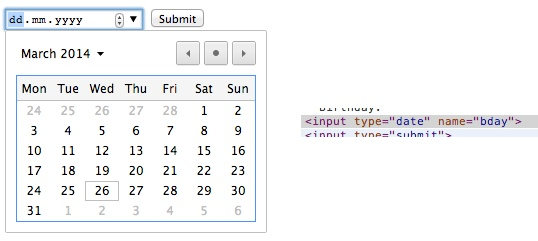
\includegraphics[]{images/datepicker.jpg}
\missingfigure{Datepicker (Visual)}
\caption[
Beispiel von Web-Components im Browser an Hand von dem Datepicker, Urldate: 04.2014 \newline
\small\texttt{https://s3.amazonaws.com/infinum.web.production/repository\_items/files/000/000/238/original/datepicker.jpg}
]{Beispiel von Web-Components im Browser an Hand von dem Datepicker}
\label{fig:3_Datepicker_Visuals}
\end{figure}

\begin{figure}[h]
\centering
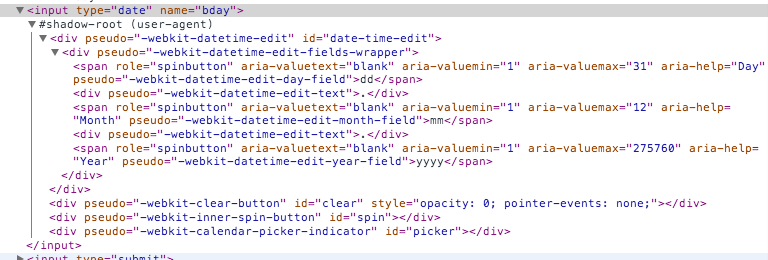
\includegraphics[height=5.0cm]{images/datepicker_shadow_dom.jpg}
\caption[
Beispiel von Web-Components im Browser an Hand von dem Datepicker, Urldate: 04.2014 \newline
\small\texttt{https://s3.amazonaws.com/infinum.web.production/repository\_items/files/000/000/236/original/datepicker\_shadow\_dom.jpg}
]{Beispiel von Web-Components im Browser an Hand von dem Datepicker}
\label{fig:3_Datepicker_Source}
\end{figure}

\textbf{Warum Web-Components?}\\
Javascript Widgets und Plugins sind fragmentiert, weil sie auf diversen unterschiedlichen Bibliotheken und Frameworks basieren, die möglicherweise nicht miteinander funktionieren. Web-Components versuchen einen gewissen Standard in Widgets und Plugins zu bringen. Das Problem der nicht miteinander funktionierenden Plugins versucht Web-Components mit Kapselung zu lösen. Durch die Lösung dieses Problems ist die Wiederverwendbarkeit von Komponenten garantiert, da es sämtliche Interferenzen\todo{richtiges Wort?} zwischen Plugins löst. Web-Components können des Weiteren viel mehr als nur UI-Komponenten sein. Eine Bibliothek könnte bereits eine Komponente darstellen, die eine gewisse Funktionalität bereitstellt.

\textbf{Unterstützung von Web-Components}\\
Zur Zeit ist die Hauptproblem von Web-Components die mangelhafte Browserunterstützung. Kein einziger Browser unterstützt diesen Standard zu 100\%. Es gibt bereits mehrere Möglichkeiten beziehungsweise Polyfills\footnote{Ein Polyfill ist ein Browser-Fallback, um Funktionen, die in modernen Browsern verfügbar sind, auch in alten Browsern verfügbar zu machen.}, um dennoch Web-Components nutzen zu können. Beispiele hierfür sind:
\begin{itemize}
\item Polyfill-Webcomponents\footnote{Mehr Information zu Polyfill-Webcomponents unter \href{http://github.com/timoxley/polyfill-webcomponents}{http://github.com/timoxley/polyfill-webcomponents}}
\item Polymer-Project\footnote{Mehr Information zu Polymer unter \href{http://www.polymer-project.org/}{http://www.polymer-project.org/}}
\item X-tags\footnote{Mehr Information zu X-tags unter \href{http://x-tags.org/}{http://x-tags.org/}}
\end{itemize}
Obwohl es mehrere Polyfills bezüglich Web-Componnts gibt, ist es egal, auf welcher Basis man seine Web-Components programmiert, denn durch die Standardisierung ist die Interkompatibilität der einzelnen Komponenten gegeben. Diese Arbeit beschränkt sich hauptsächlich auf die Entwicklung von Web-Components mit Hilfe des Standards beziehungsweise der Polyfill-Bibliothek Polymer.\\
Durch die Benutzung von dem Polyfill Polymer funktionieren Web-Component in allen \glqq evergreen\grqq -Browsern\footnote{Ein \glqq Evergreen\grqq -Browser ist ein Web-Browser, der sich automatisch beim Start updatet.} und Internet-Explorer 10 und neuer. Des Weiteren funktionieren sie dadurch auf mobilen Endgeräten, wo iOS6+, Chrome Mobile, Firefox Mobile, oder Android 4.4 oder höher vorhanden ist. Auch mit Hilfe von Polyfill bieten sowohl der Internet-Explorer 9 und niedriger, als auch Android-Browser 4.3 oder niedriger keine Unterstützung für Web-Components. Dies bedeutet, dass Web-Components zur Zeit noch für die Verwendung im Web bereit sind, außer man hat als Zielgruppe ausschließlich eine Plattform, die unterstützt wird.

\textbf{Web-Components Alternativen}
Die folgenden Alternativen von Web-Components benutzen ähnliche Patterns um die gewünschte DOM-Abstrahierung zu erreichen.
\begin{description}
\item[React] benutzt seinen eigenen \glqq Virtual DOM\grqq und versucht in keinster Hinsicht Web-Components zu simulieren. Folglich ist die Browser-Unterstützung von React besser, als jene der Web-Components. Ab Internet-Explorer 8 werden sämtliche Browser vollständig unterstützt. Zur Zeit wird diese Technologie in Facebooks und Instagrams Kommentarsystemen eingesetzt.
\item[AngularJS] besitzt diverse Interferenzen zu Web-Components, jedoch versucht auch diese Technologie nicht Web-Components zu simulieren, um bessere Browser-Unterstützung zu bieten (Internet Explorer 8+). Die genaue Unterscheidung bezüglich AngularJS-Direktiven und Web-Components werden in Kapitel \ref{sec:3_Polymer} auf Seite \pageref{sec:3_Polymer} erklärt.
\end{description}
